\chapter{Analyse et Conception}

\section{Introduction}
Le but de ce chapitre est de faire un cadrage technique et fonctionnel de notre projet. Nous allons présenter la démarche du de conception suivie, les besoins fonctionnels et non fonctionnels de notre projet, ainsi les diagrammes de cas d'utilisation réalisés.



\section{Besoin fonctionnels}
Il s’agit des fonctionnalités du système. Ce sont les besoins spécifiant un comportement d’entrée / sortie du système.

Afin d’obtenir une vue globale sur les exigences de l’application et ainsi réussir une bonne spécification des besoins, ces derniers doivent être modélisés. Nous avons donc eu recours aux concepts d’UML (Unified Modeling Language) pour représenter l'architecture et le fonctionnement de différentes fonctionnalités grâce à un ensemble de diagrammes très explicites.

\section{Besoin non fonctionnels}
Il s’agit des besoins qui caractérisent le système. Ce sont des besoins en matière de performance, de type de matériel ou le type de conception. Ces besoins peuvent concerner les contraintes d’implémentation. Ils agissent de façon indirecte sur le résultat et sur le rendement de l’application, ce qui fait qu’ils ne doivent pas être négligés, pour cela il faut répondre aux exigences suivantes :

\subsection{Fiabilité :}
La plateforme doit fonctionner de façon cohérente sans erreurs et doit être satisfaisante.
\subsection{Les erreurs :}
Les ambigüités doivent être signalées par des messages d’erreurs bien organisés pour bien guider l’utilisateur et le familiariser avec notre application.
\subsection{Ergonomie et bonne interface :}
L’application doit être adaptée à l’utilisateur dans toutes les résolution d’écran sans qu’il ne fournisse aucun effort (utilisation claire et facile) de point de vue navigation entre les différentes pages, couleurs et mises en textes utilisés.
\subsection{Sécurité :}
Notre solution doit respecter surtout la confidentialité des données personnelles des clients qui reste l’une des contraintes les plus importantes dans ces plateformes.
\subsection{Aptitude à la maintenance et la réalisation :}
Le système doit être conforme à une architecture standard et claire permettant sa maintenance et sa réutilisation.




\section{Diagramme de cas d'utilisation} \\
Les diagrammes de cas d'utilisation modélisent le comportement d'un système et permettent de capturer ses exigences. Ils décrivent aussi les fonctions générales et la portée d'un système.
\begin{figure}[!h]
\begin{center}
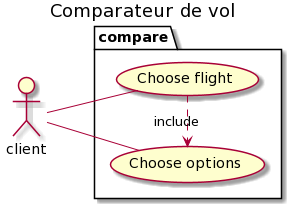
\includegraphics[height=8cm]{Pictures/Use case.png}
\end{center}
\caption{Diagramme de cas d'utilisation}
\end{figure}

\newpage
\section{Diagramme de classe}
Le diagramme de classes représente les classes intervenant dans le système. Le diagramme de classes est une représentation statique des éléments qui composent un système et de leurs relations

\begin{figure}[!h]
\begin{center}
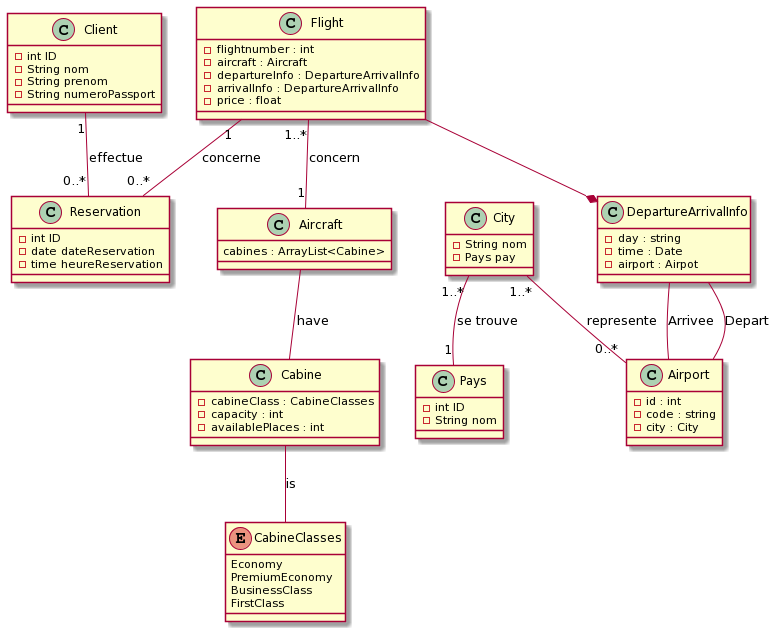
\includegraphics[height=8cm]{Pictures/Diag de classe.png}
\end{center}
\caption{Diagramme de classe}
\end{figure}
\section{Conclusion}

\\ L’analyse fonctionnelle est une démarche qui consiste à rechercher et à caractériser les fonctions offertes par un produit pour satisfaire les besoins de son utilisateur. Ce chapitre nous a permis de bien décrire le comportement de notre projet du point de vue de l’utilisateur en étudiant les besoins fonctionnels et non fonctionnels ainsi les diagrammes Classes et Cas d'utilisation.